\documentclass[../structure.tex]{subfiles}
%\usepackage{../mypkg}
\begin{document}
\chapter{Method and Implementation}
\hspace{2em}As we are implementing registration method, we are going to consider two objects, Target Graph $T$, which is remain fixed, and Template Graph $S$, which moves iteratively until it reach the optimal alignment with target graph $T$. To do so, we use Iterative Closest Point (ICP) as we mentioned before (see figure [\ref{fig:icp}]), for each point on template graph $S$ we look for closest point on target graph $S$. Then we start moving each point in $S$ to correspondent point in $T$ with respect to stiffness. After solving the cost function by using \textit{Least Square (LSQR)} we have separate \textit{Affine Transformation Matrix} ($X = [x_{1}, x_{2}, x_{3}, ...,x_{n}]$) for each point in the template graph $S$ that moves separately whiles keep the original neighbors close to each other as possible. This type of registration is called non-rigid registration.

\begin{figure}[h!]
\centering
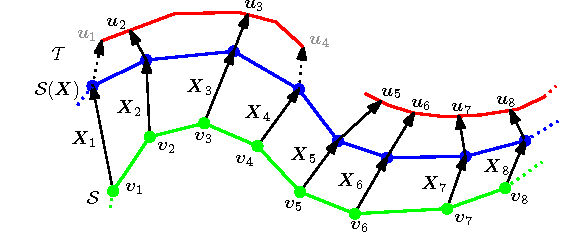
\includegraphics[scale=0.5]{001_conn}
\captionsetup{justification=centering}
\caption{The template graph $S$ (green) is deformed by locally affine transformations $(X_{i})$ onto the target graph $T$ (red). The algorithm determines closest points $(u_{i})$ for each displaced source vertex $(X_{i}v_{i})$ and finds the optimal deformation for the stiffness used in this iteration. This is repeated until a stable state is found. The process then continues with a lower stiffness. Due to the stiffness constraint the vertices do not move directly towards the target graph, but may move parallel along it. The correspondences $u_{1}$
and $u_{4}$ are dropped as they lie on the border of the target \cite{Amberg2007}.}
\label{fig:icp}
\end{figure}

\section{Data preparation}
\hspace{2em}In this thesis we follow the method in \cite{Amberg2007} which is implemented for surface graphs, but due to differences between data used in \cite{Amberg2007} which is surface graphs saved in points cloud format or mesh format, and our data which is pathways in streamlines format saved in \textit{ply} file as shown in figure [\ref{fig:data}], therefore  we had to build a tool for reading \textit{ply} file format as streamlines and build graphs out of it, each \textit{ply} file has one pathway.

\begin{figure}[h!]
\centering
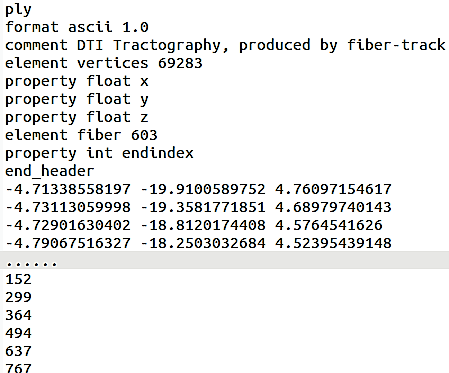
\includegraphics[scale=0.5]{002_data}
\captionsetup{justification=centering}
\caption{A sample of a Brain pathway saved in a \textit{ply} file.}
\label{fig:data}
\end{figure}

\subsection{The PLY file}
\hspace{2em}Let us illustrate a bit our data and \textit{ply} files we used to save our data as shown in figure [\ref{fig:data}]. It consist of two parts, header and body. The header consist of all information that necessary to pars the file, and the body has the data itself.
\begin{itemize}
\item The first line represent the file type.
\item The second line is the file format.
\item The third line is comment.
\item The forth line is first group of elements (as \textit{ply} can have many) name and number (each element in one line). It shows that we have 69283 vertices.
\item The 5th, 6th and 7th lines shows that the first group of elements has three properties, each of them in float format and the name of each property.
\item The 8th line shows the second group of elements which has 603 fiber tract and so on.
\item The 10th line shows the end of the header part.
\item The remaining lines is the body of the file which has all the data, each element in one line.
\end{itemize}

\hspace{2em}Before we start registering the graphs, it is better to have the initial position which makes the template graph $S$ as close as possible to the target graph $T$ and in the best possible alignment before ICP. To do so, we use Principal Components Analysis (PCA) which illustrated down below.

\section{Principal Components Analysis (PCA)}
\hspace{2em}Before applying PCA, we scale the template graph $S$ and the target graph $T$ to a $[0,1]$ scale to match each other. This is done by subtracting all points from the minimum value in the graph and then dividing them by the maximum value in the graph. Next, we apply PCA and use $[-1,1]^3$ cube combination and measure the euclidean distance between each point in the template graph to the closest point in the target graph $\sum ||v_i-v_j||_F^2$ where $v_i \in S, v_j \in T$ eight times to select the combination with the minimum distance as is illustrated in table \{\ref{table:cube}\} and in figure [\ref{fig:pca}] .
\vspace{2em}
\begin{center}
\begin{table}[h]
	\begin{tabular}{| c | c | c | c | c | c | c | c |}
	\hline
	1 & 2 & 3 & 4 & 5 & 6 & 7 & 8\\
	\hline
	(x,y,z) & (x,y,-z) & (x,-y,z) & (x,-y,-z) & (-x,-y,z) & (-x,y,-z) & (-x,y,z) & (-x,-y,-z)\\
	\hline
	\end{tabular}
\caption{$[-1,1]^3$ cube combination}
\label{table:cube}
\end{table}
\end{center}
\vspace{2em}
\begin{figure}[h!]
	\centering
	\begin{subfigure}[b]{0.59\textwidth}
	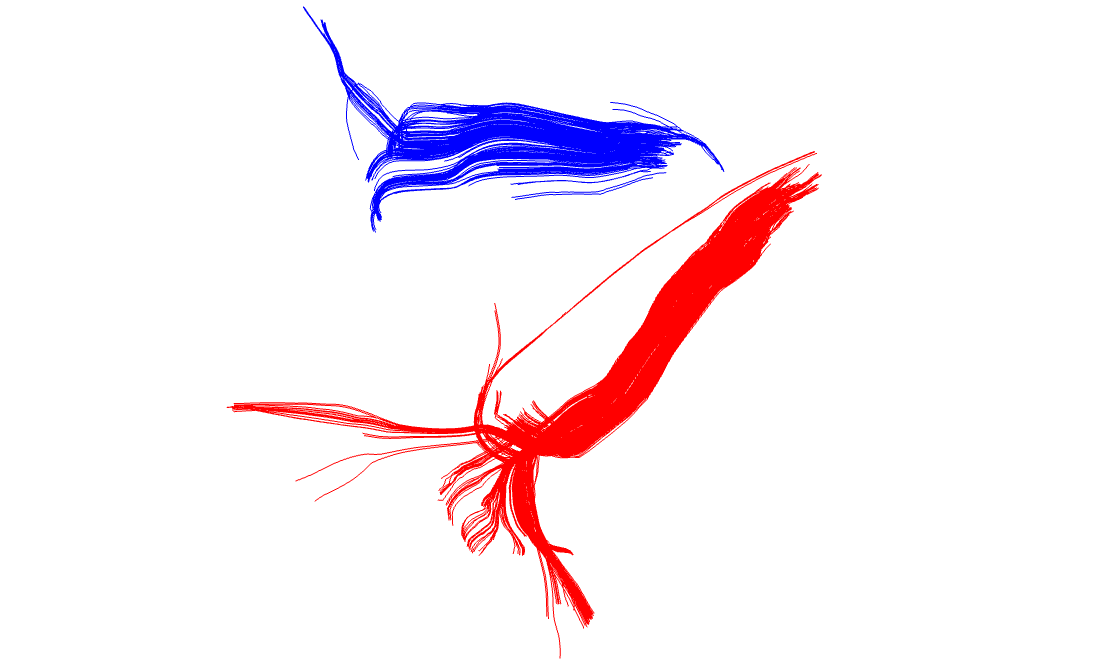
\includegraphics[width=\textwidth]{003_original}
	\caption{Original position}
	\end{subfigure}
	% separate
	\begin{subfigure}[b]{0.39\textwidth}
	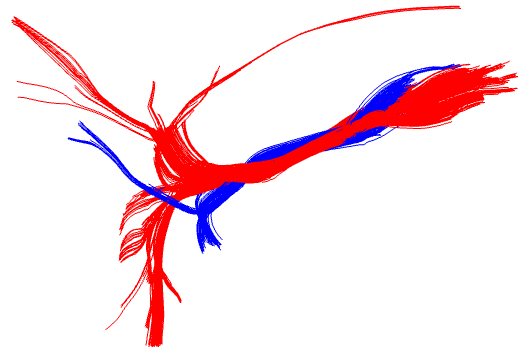
\includegraphics[width=\textwidth]{004_pca}
	\caption{After PCA}
	\end{subfigure}
\caption{Applying PCA for initial alignment before ICP}
\label{fig:pca}
\end{figure}

\vspace{2em}
\section{Cost Function}
\hspace{2em}The simplest form of the cost function is shown in the equation (\ref{equ:equation1}):

\begin{equation}
\label{equ:equation1}
||Ax-b||^2
\end{equation}

This simple form of the cost function makes it easy to solve by \textit{Least Square (LSQR)} (\textit{scipy.sparse.linalg.lsqr}) algorithm which is implementation of a conjugate-gradient type method for solving sparse linear equations and sparse least-squares problems \cite{Paige1982a}.

To illustrate the cost function more we need to divide it to three parts as shown in equation (\ref{equ:costFun}), distance term, stiffness term, and landmark term.

\begin{equation}
E(X) = E_{d}(X) + \alpha E_{s}(X) + \beta E_{t}(X)
\label{equ:costFun}
\end{equation}

\subsection{Distance Term}
\hspace{2em}The first part of the cost function (\ref{equ:costFun}) is the distance term, it represent the summation of distances between each point in the template graph $S$ and it is correspondent point in target graph $T$ which illustrated in equation (\ref{equ:distance1}):

\begin{equation}
E_{d}(X) = \sum_{v_{i} \in V} w_{i}dist^2(T,x_{i}v_{i})
\label{equ:distance1}
\end{equation}

where $W = [w_{1}, w_{2}, w_{3}, ..., w_{n}];\quad w_{i}\in [0,1]$ is weight which is \textit{one} if the correspondent point distance is below the threshold and \textit{zero} if not, even some points in template graph do not have correspondences in target graphs $T$, they move with their neighbors due to stiffness term. $T$ is the target graph, $x_{i}$ is the correspondent affine matrix in size $3\times4$, $v_{i}\in V$ is template graph $S$ vertex in homogeneous coordinates $v_{i} = [x,y,z,1]$ because we want to include transformation on affine matrix $x_{i}$ and the distance between each point in the template graph $S$ and its closest point in target graph $T$ is represented by $dist^2(T,x_{i}v_{i})$.

\subsection{Stiffness Term}
\hspace{2em}The stiffness term is the second part of the equation (\ref{equ:stiffness1}), it is the part of the equation regularizes the deformation by penalizing the weighted difference of the transformations of neighboring vertices under the Frobenius norm $||.||_{F}$ using a weight matrix $G := diag(1, 1, 1, \gamma)$ \cite{Amberg2007}, that keeps the vertices which are linked together (i.e., there is an edge between them or they are in the same tract) or neighbors close to each other.

\begin{equation}
E_{s}(X) = \sum_{i,j \in E} ||(X_{i} - X_{j})G||_{F}^2
\label{equ:stiffness1}
\end{equation}

The parameter $\gamma$ is used to balance the rotational and skew  against translation while transforming the template graph $S$ \cite{Amberg2007}. In our case $\gamma$ is \textit{one} as we have already scaled our data into the $[-1, 1]^3$ cube.

To make our function solvable directly we need to write it as quadratic function, therefore we use twelve parameters per vertex in $3 \times 4$ shape. The part $||.||_{F}$ is the \textit{Frobenius norm} which illustrated in the example below (\ref{equ:stiffness2}) \cite{Amberg2007}: 

\begin{equation}
||A||_{F} = \sqrt{\sum_{i=1}^m \sum_{j=1}^n |a_{ij}|^2}
\label{equ:stiffness2}
\end{equation}

The $\alpha$ parameter in equation (\ref{equ:costFun}) is a constant that manages the effect of the stiffness term; when it is high the neighbor vertices does not move far from eachother and when it is low, a greater deformation can occur.

\subsection{The Landmark Term}
\hspace{2em}The landmark term gives the initial position of the template graph $S$ shown in equation (\ref{equ:landmark1}) below:

\begin{equation}
E_{l}(X) = \sum_{(vi,l) \in L}||(X_{i}v_{i} - l)||^2
\label{equ:landmark1}
\end{equation}

Where $L = \left\{(v_{i1},l_{1}),(v_{i2},l_{2}),...,(v_{il},l_{l})\right\}$ is the set of landmarks that maps the template graph $S$ to the target graph $T$.



\end{document}